\documentclass{beamer}

\useoutertheme[subsection=false]{miniframes}
\usecolortheme{beaver}
\setbeamertemplate{navigation symbols}{}
\setbeamertemplate{footline}{}
\usepackage{graphicx}
\usepackage{url}
\usepackage{datetime}
\usepackage{tikz-cd}
\newcommand{\lectureDate}{\formatdate{23}{10}{2018}}

\setbeamertemplate{caption}
{\raggedright\insertcaption\par}
\title{MATH211: Linear Methods I}
\author{Matthew Burke}
\date{\lectureDate}
\begin{document}

\frame{\titlepage}

\begin{frame}{Lecture on \lectureDate}
  \tableofcontents
\end{frame}

\section*{Last time}
\label{sec:Last-time}

\begin{frame}{Last time}
  \begin{itemize}
  \item Closest points\vfill
  \item Examples\vfill
  \item Cross product
  \end{itemize}
\end{frame}

\begin{frame}{Review midterm material}
\begin{itemize}
  \item Practice questions:
  \begin{itemize}
    \item Past exams: d2l > Content > Midterm and Final Exam
    \item Lab questions
    \item Exercises in lectures
    \item d2l > Content > Additional course material > Additional practice problems
    \item Exercises from textbook
  \end{itemize}
  \item Core material:
  \begin{enumerate}
    \item Row reduction algorithm
    \begin{itemize}
      \item And formulation in terms of elementary matrices
    \end{itemize}
    \item Inversion algorithm
    \begin{itemize}
      \item And formulation in terms of elementary matrices
    \end{itemize}
    \item Determinant by row/column operations
    \begin{itemize}
      \item And formulation in terms of elementary matrices
    \end{itemize}
  \end{enumerate}
	\item Clarify material from lectures 2018-10-02 and 2018-10-04
\end{itemize}
\end{frame}

\section{Cross product}

\begin{frame}
\begin{beamercolorbox}[sep=12pt,center]{part title}
\usebeamerfont{section title}
\insertsection\par
\end{beamercolorbox}
\end{frame}

\begin{frame}{Trigonometric definition of cross product}
\begin{columns}
  \column{0.5\textwidth}
  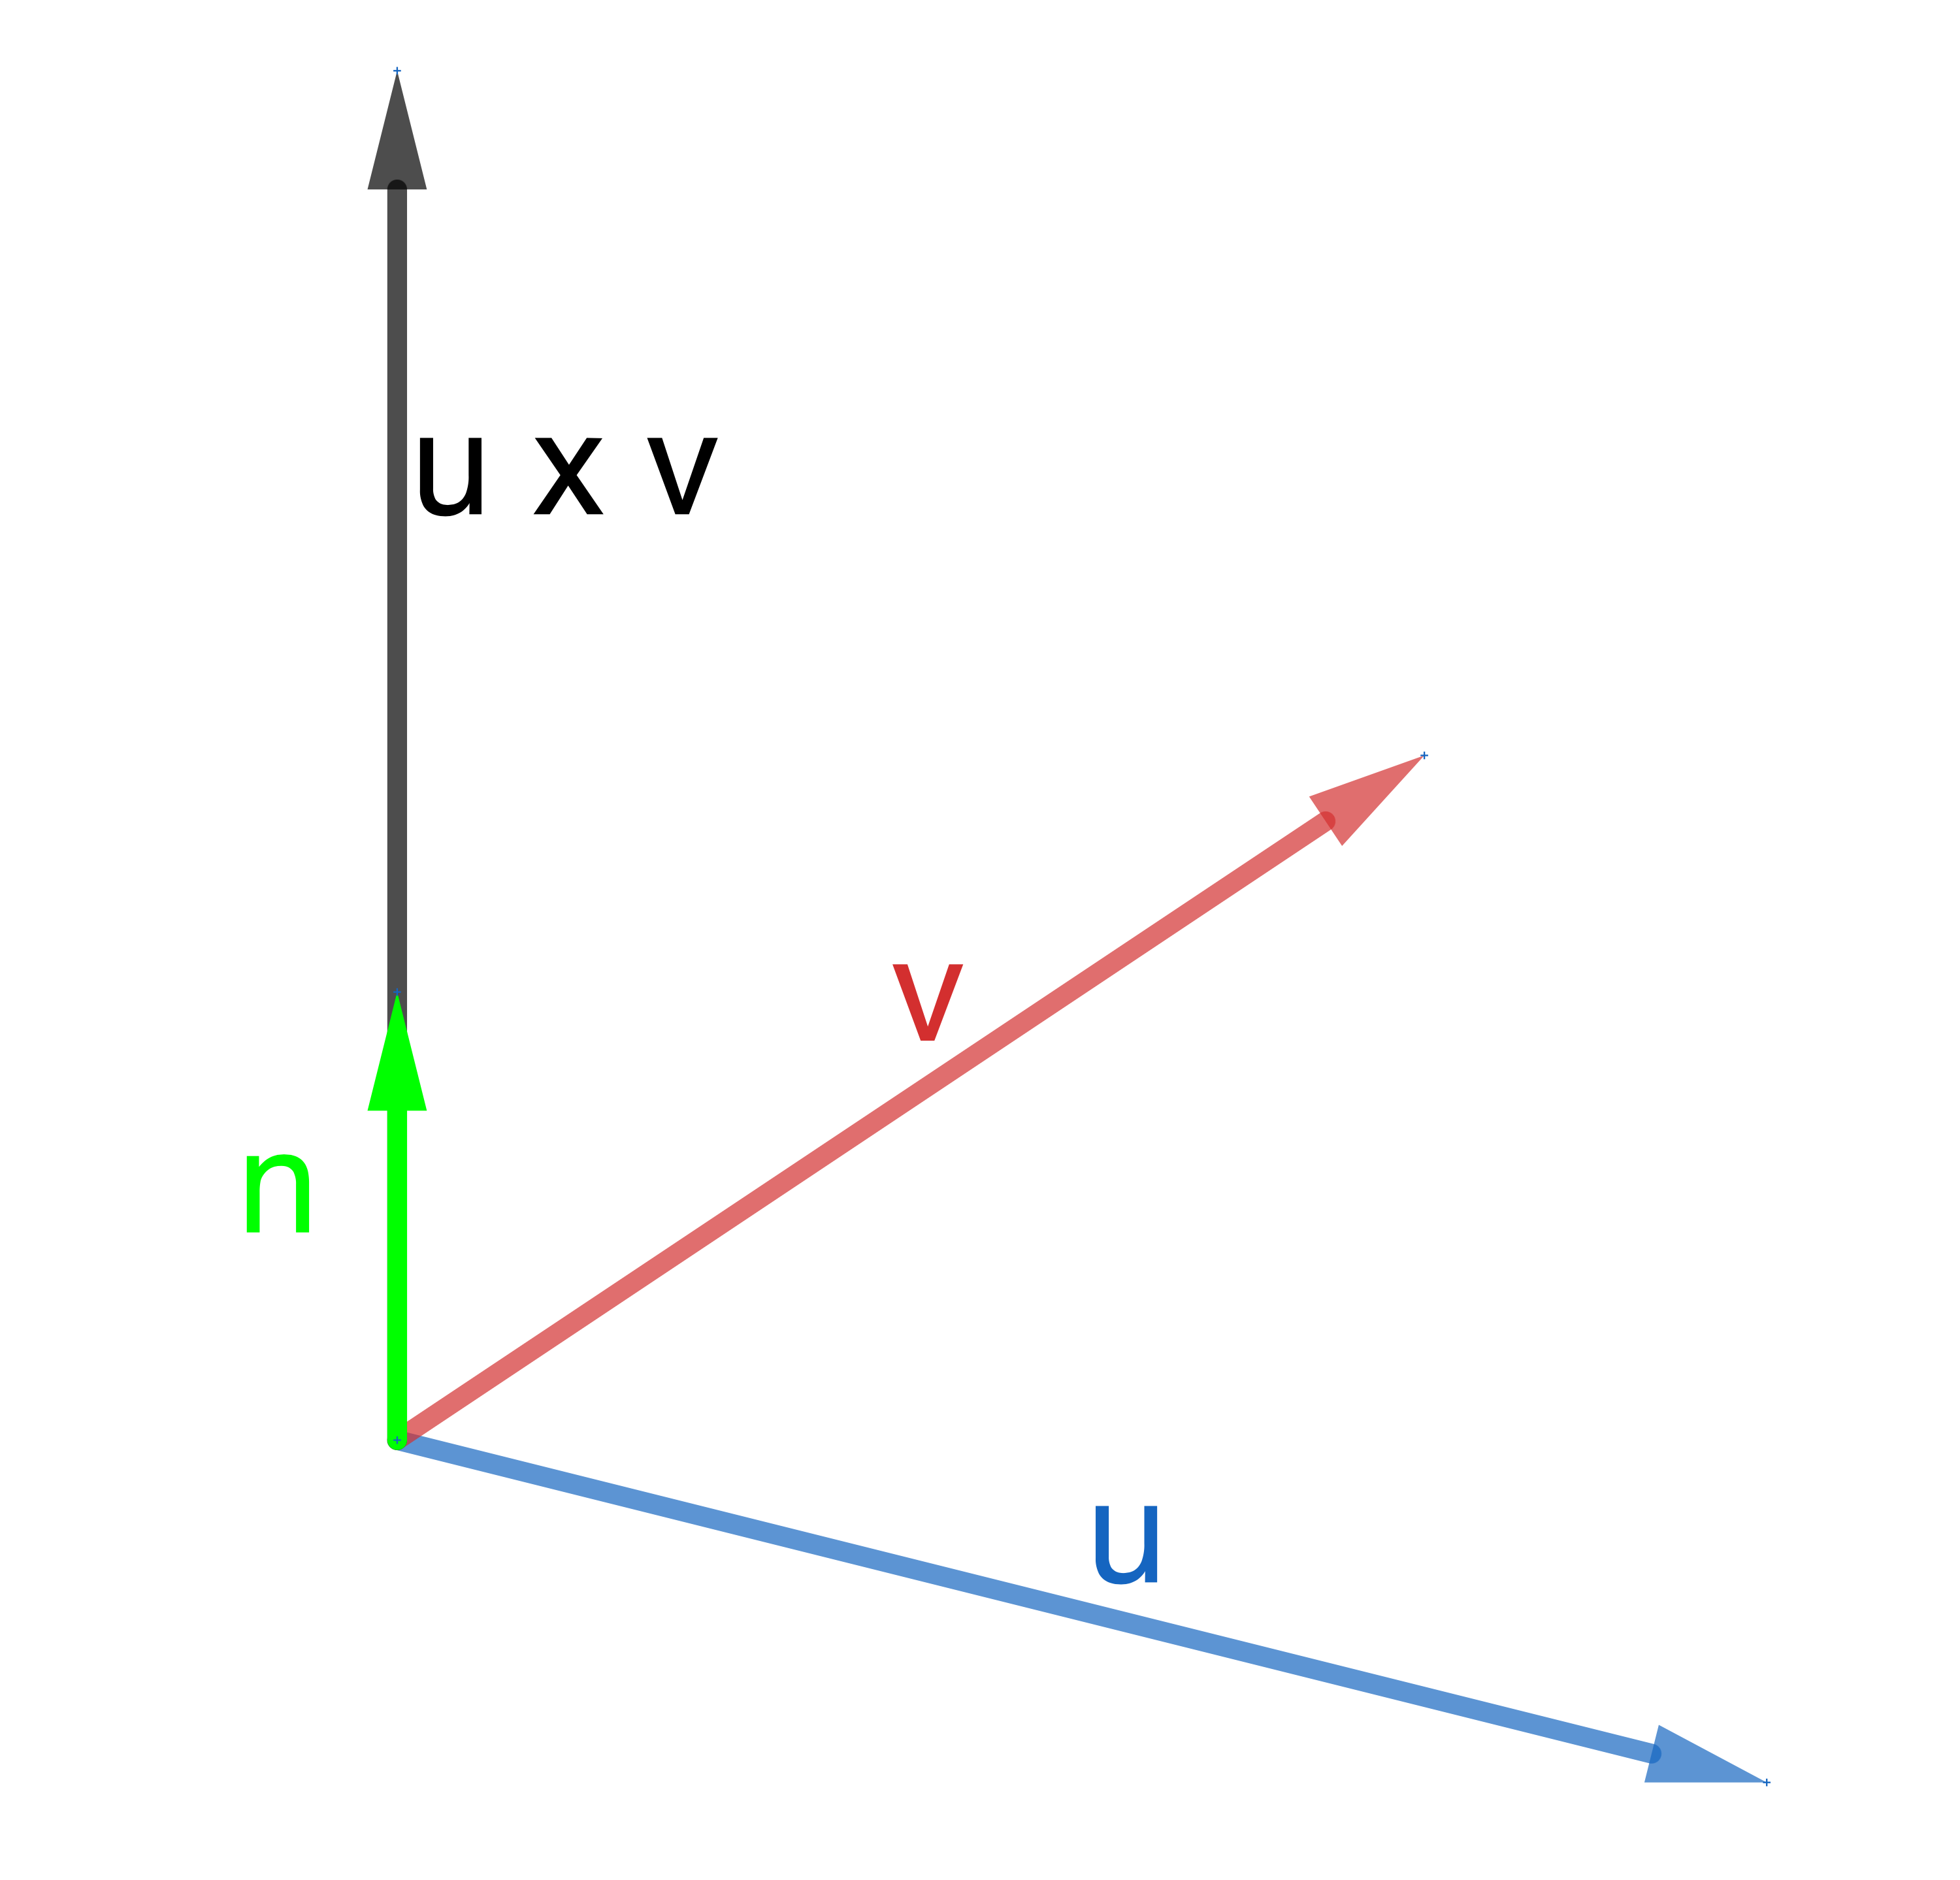
\includegraphics{cross-product-direction.png}
  \column{0.5\textwidth}
  Alternatively:
  \begin{equation*}
  u\times v = \|u\|\|v\| sin\theta n
  \end{equation*}
  where $n$ is a unit vector orthogonal to both $v$ and $u$.\vfill
  {\bf Aide-memoire:}
  \begin{equation*}
  \left[
  \begin{array}{c}
  1\\
  0\\
  0
  \end{array}
  \right]\times \left[
  \begin{array}{c}
  0\\
  1\\
  0
  \end{array}
  \right] = \left[
  \begin{array}{c}
  0\\
  0\\
  1
  \end{array}
  \right]
  \end{equation*}
\end{columns}
\end{frame}

\begin{frame}{Cross product on standard basis vectors}
If 
\begin{equation*}
e_1 = \left[
  \begin{array}{c}
  1\\
  0\\
  0
  \end{array}
  \right],
  e_2 = \left[
  \begin{array}{c}
  0\\
  1\\
  0
  \end{array}
  \right],
  e_3 = \left[
  \begin{array}{c}
  0\\
  0\\
  1
  \end{array}
  \right]
\end{equation*}
then 
\begin{align*}
e_1\times e_1 = 0 && e_1\times e_2 = e_3 && e_1\times e_3 = -e_2\\
e_2\times e_1 = -e_3 && e_2\times e_2 = 0 && e_2\times e_3 = e_1\\
e_3\times e_1 = e_2 && e_3\times e_2 = -e_1 && e_3\times e_3 = 0
\end{align*}
\end{frame}

\begin{frame}{Algebraic definition of cross product}
So in general:
\begin{equation*}
u\times v = \left[
\begin{array}{c}
u_1\\
u_2\\
u_3
\end{array}
\right]\times \left[
\begin{array}{c}
v_1\\
v_2\\
v_3
\end{array}
\right] =
\left(u_1e_1+u_2e_2+u_3e_3\right)\times \left(v_1e_1+v_2e_2+v_3e_3\right)
\end{equation*}
\begin{align*}
=&u_1v_1(e_1\times e_1) && +u_1v_2(e_1\times e_2)  && +u_1v_3(e_1\times e_3) \\
&+u_2v_1(e_2\times e_1) && +u_2v_2(e_2\times e_2) && +u_2v_3(e_2\times e_3 )\\
&+u_3v_1(e_3\times e_1)  && +u_3v_2(e_3\times e_2)  && +u_3v_3(e_3\times e_3)
\end{align*}
\begin{align*}
=&0 && +u_1v_2e_3  && -u_1v_3e_2 \\
&-u_2v_1e_3 && +0 && +u_2v_3e_1\\
&+u_3v_1e_2  && -u_3v_2e_1  && +0
\end{align*}
\end{frame}

\begin{frame}{Algebraic definition}
\begin{definition}
The \emph{cross product $u\times v$ of $u$ with $v$} is
\begin{equation*}
u\times v = \left[
\begin{array}{c}
u_1\\
u_2\\
u_3
\end{array}
\right]\times \left[
\begin{array}{c}
v_1\\
v_2\\
v_3
\end{array}
\right] = \left[
\begin{array}{c}
u_2v_3-u_3v_2\\
u_3v_1-v_3u_1\\
u_1v_2-u_2v_1
\end{array}
\right]
\end{equation*}
\end{definition}
The following heuristic doesn't make sense formally but may be an easier way to remember.
\begin{equation*}
	\vec{u}\times\vec{v} =
	\left|\begin{array}{ccc}
	\vec{i} & \vec{j} & \vec{k} \\
	u_1 & u_2 & u_3 \\
	v_1 & v_2  & v_3 
	\end{array}\right|,
	\mbox{ where }
	\vec{i} = 
	\left[\begin{array}{c}
	1 \\ 0 \\ 0 \end{array}\right],
	\vec{j} = 
	\left[\begin{array}{c}
	0 \\ 1 \\ 0 \end{array}\right],
	\vec{k} = 
	\left[\begin{array}{c}
	0 \\ 0 \\ 1 \end{array}\right].
\end{equation*}
\end{frame}

\begin{frame}{Properties of the cross product}
\begin{theorem}
Let $\vec{u}, \vec{v}$ and $\vec{w}$ be in $\mathbb{R}^3$.
\begin{enumerate}
\item $\vec{u}\times\vec{0}=\vec{0}$ and
$\vec{0}\times\vec{u}=\vec{0}$.
\item $\vec{u}\times\vec{u}=\vec{0}$.
\item $\vec{u}\times\vec{v} = - (\vec{v}\times\vec{u})$.
\item $(k\vec{u})\times\vec{v}
= k(\vec{u}\times\vec{v})
=\vec{u}\times(k\vec{v})$ for any scalar $k$.
\item $\vec{u}\times(\vec{v} + \vec{w}) =
\vec{u}\times\vec{v} + \vec{u}\times\vec{w}$.
\item $(\vec{v} + \vec{w})\times\vec{u}=
\vec{v}\times\vec{u} + \vec{w}\times\vec{u}$.
\end{enumerate}
\end{theorem}
\end{frame}

\begin{frame}{Example}
\begin{example}
  Find $u\times v$ where
  \begin{equation*}
  u= \left[
  \begin{array}{c}
  1\\
  -1\\
  2
  \end{array}
  \right]\text{ and } v = \left[
  \begin{array}{c}
  3\\
  -2\\
  1
  \end{array}
  \right]
  \end{equation*}
\end{example}
\begin{example}
Find all vectors orthogonal to 
\begin{equation*}
\left[
\begin{array}{c}
1\\
-3\\
2
\end{array}
\right]\text{ and } \left[
\begin{array}{c}
0\\
1\\
1
\end{array}
\right]
\end{equation*}
\end{example}
\end{frame}

\begin{frame}{Examples}
\begin{example}
  Give a non-parametric equation for the plane passing through
  \begin{equation*}
  \left[
  \begin{array}{c}
  1\\
  -1\\
  2
  \end{array}
  \right]\text{ , } \left[
  \begin{array}{c}
  2\\
  0\\
  -1
  \end{array}
  \right]\text{ and }
  \left[
  \begin{array}{c}
  0\\
  -2\\
  3
  \end{array}
  \right]
  \end{equation*}
\end{example}
\end{frame}

\section{Applications}

\begin{frame}
\begin{beamercolorbox}[sep=12pt,center]{part title}
\usebeamerfont{section title}
\insertsection\par
\end{beamercolorbox}
\end{frame}

\begin{frame}{Cross product and projection}
\begin{columns}
\hspace{-1.5cm}
	\column{0.5\textwidth}

	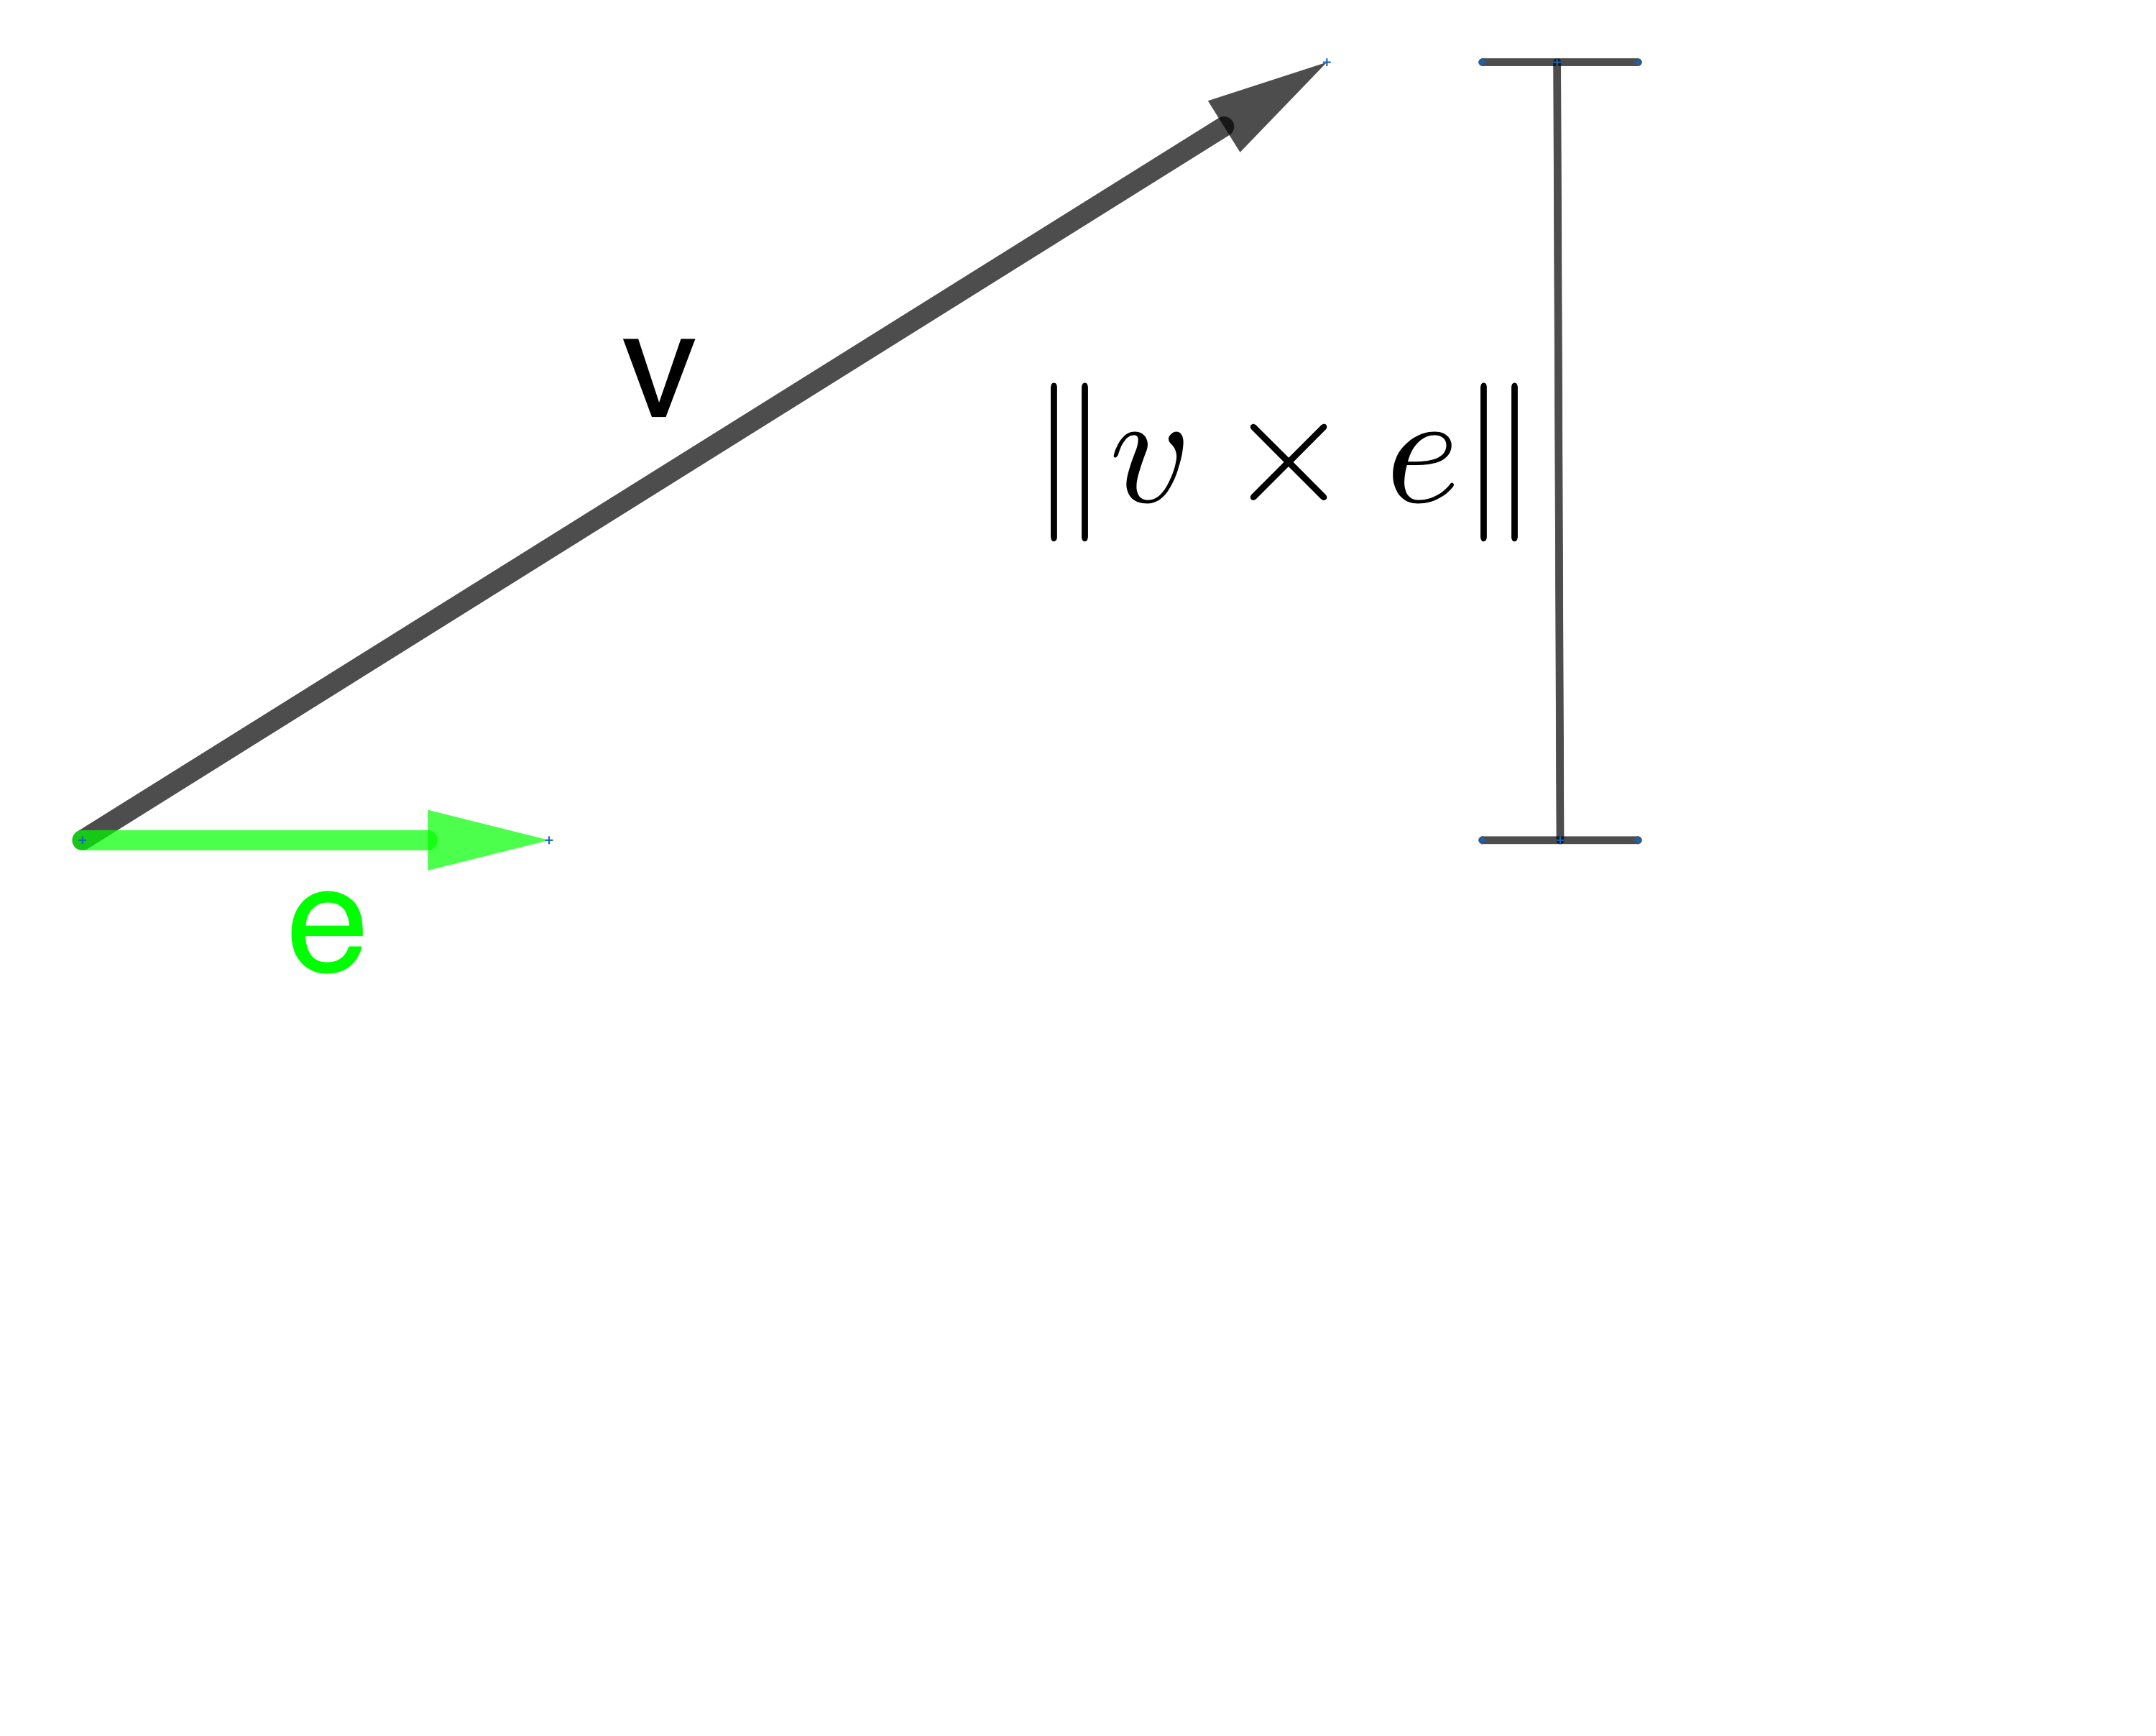
\includegraphics[scale=0.5]{cross-projection.png}
	\column{0.4\textwidth}
	If $e$ is a unit vector then
	\begin{equation*}
	\|v\times e\| = \|v\|\|e\| sin\theta = \|v\|sin\theta
	\end{equation*}
	which is the distance from the tip of $v$ to the line in direction $e$.
\end{columns}
\end{frame}

\begin{frame}{Line given by parametric equations}
    \begin{columns}
        \hspace{-1cm}
        \column{0.5\textwidth}
        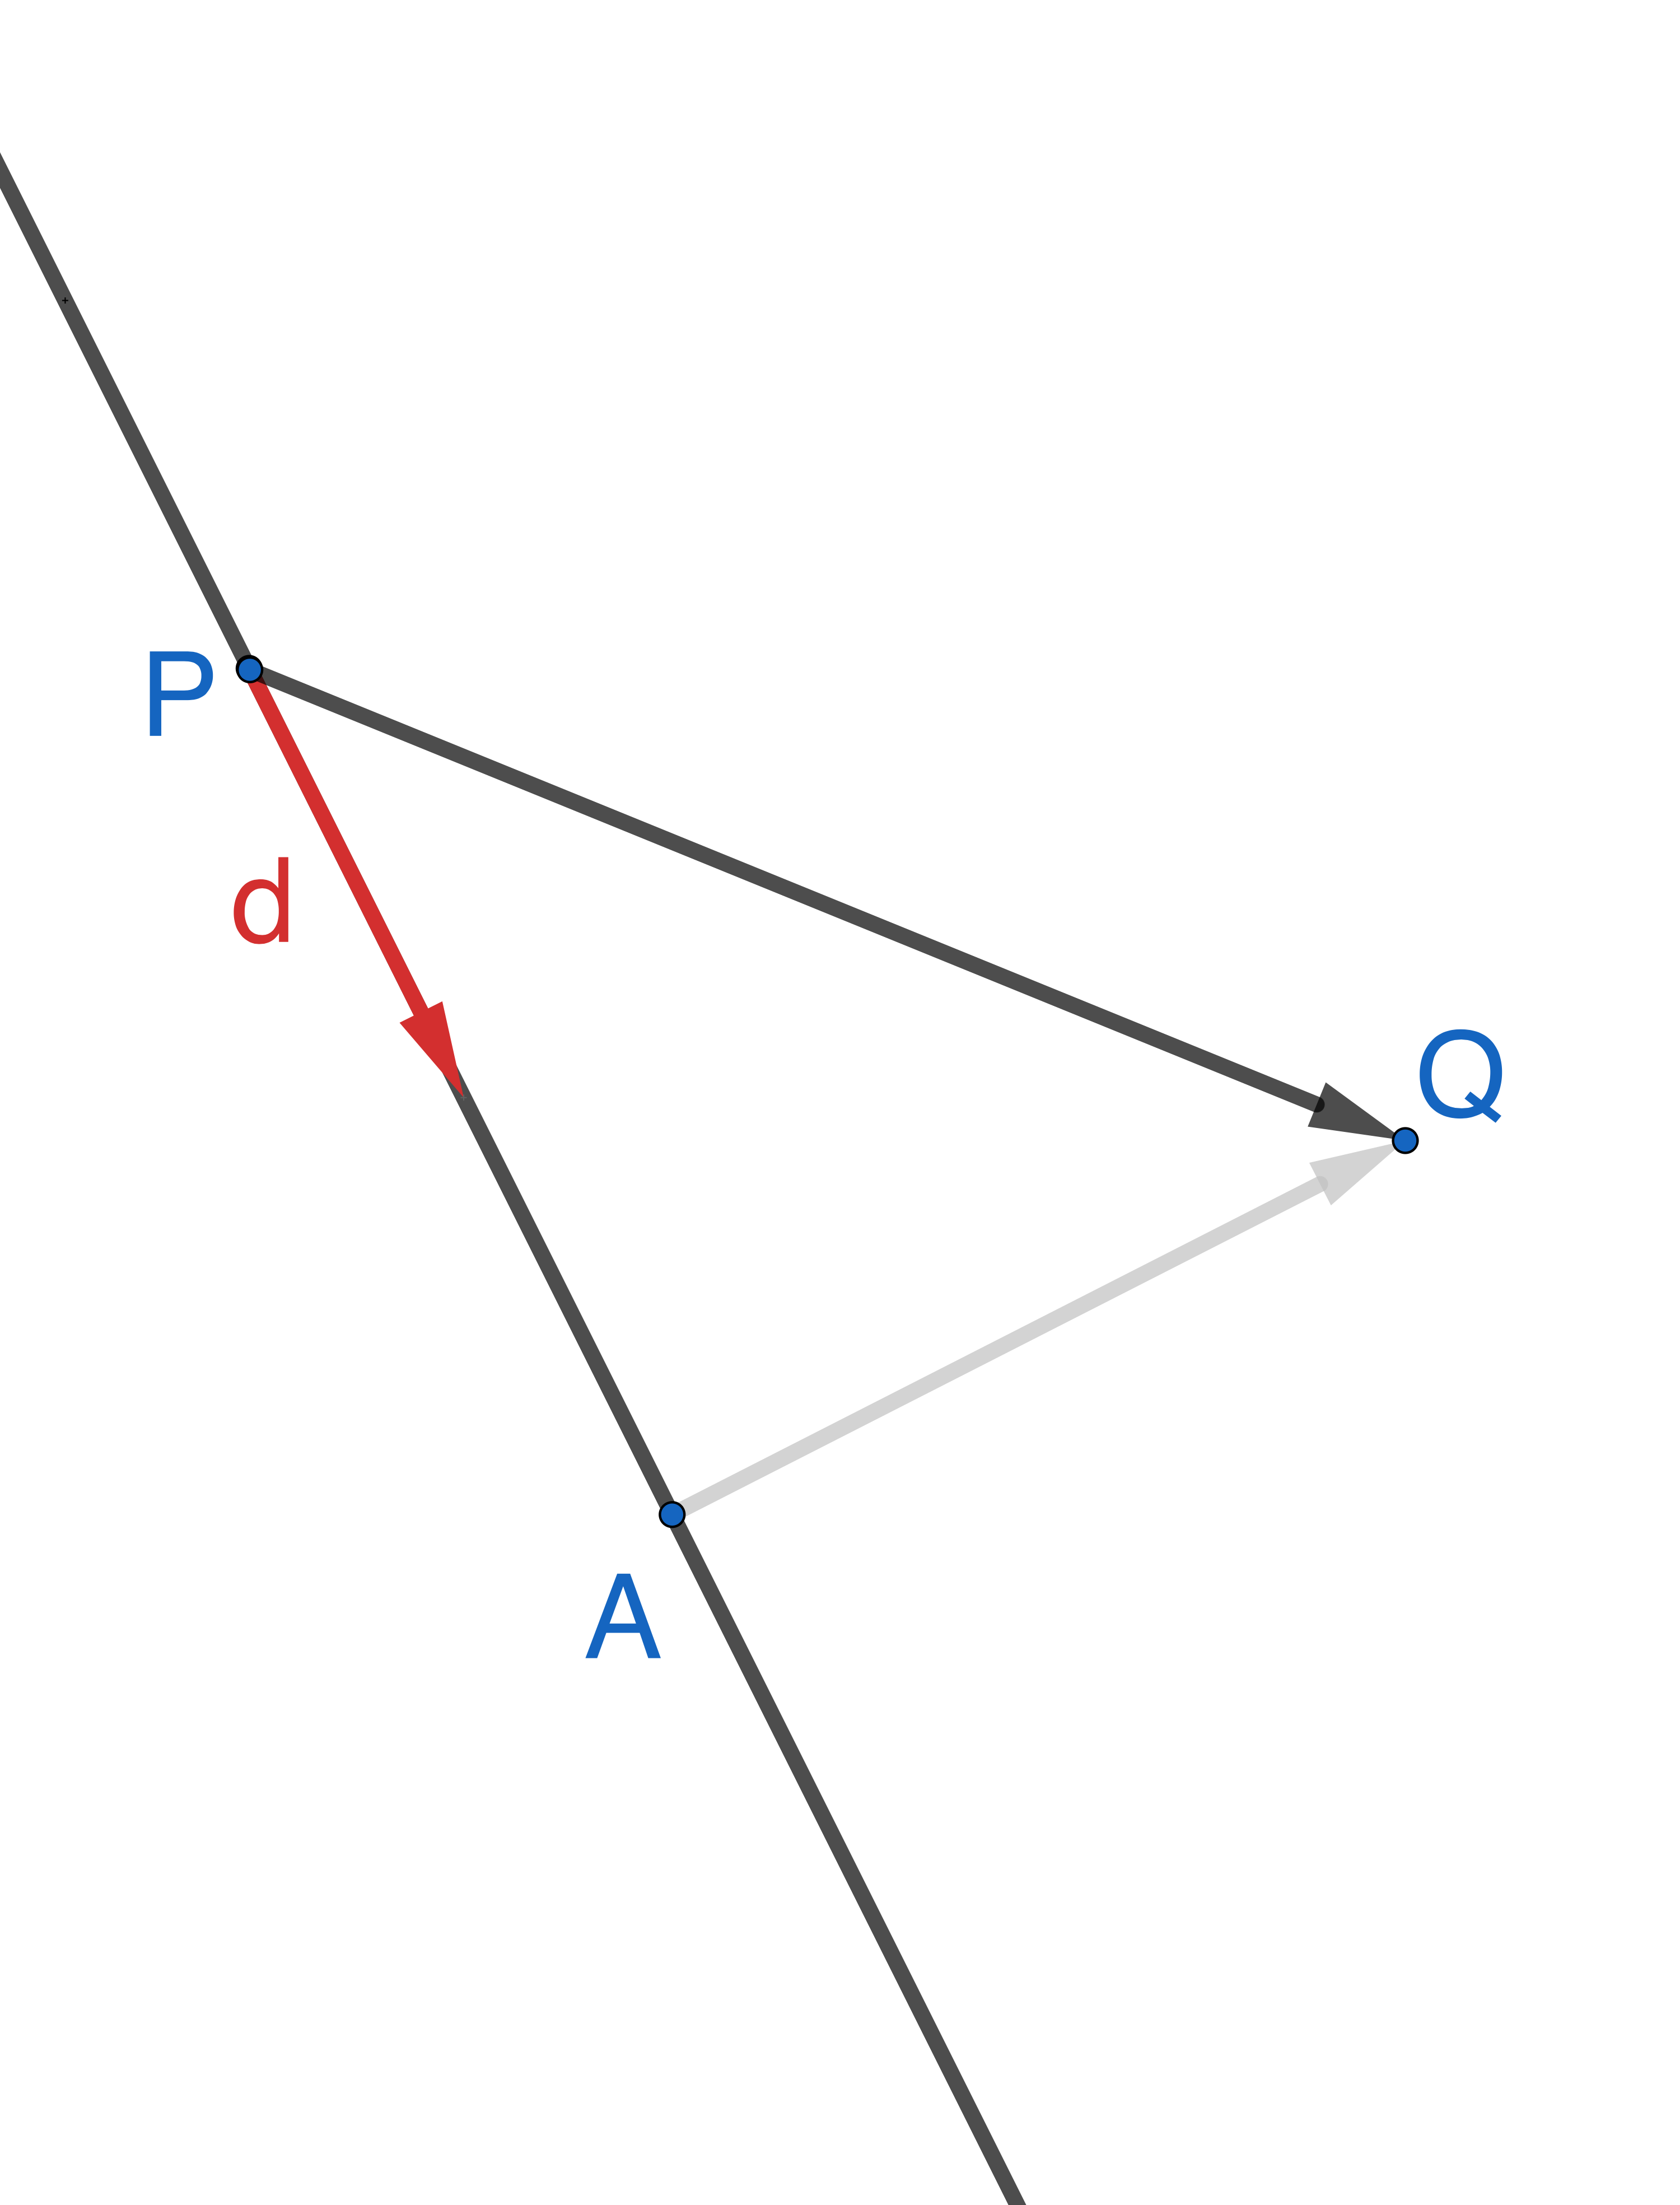
\includegraphics[scale=0.6]{2d-parametric-closest.png}
        \column{0.4\textwidth}
        If we only require the distance from $Q$ to the line \emph{and are in $\mathbb{R}^3$}:
        \begin{align*}
        d(A, Q)&= \left\|\frac{d}{\|d\|}\times \overrightarrow{PQ}\right\|\\
        &= \frac{\|d\times(Q-P)\|}{\|d\|}
        \end{align*}
        (Technique only works in $\mathbb R^3$.)
    \end{columns}
\end{frame}

\begin{frame}{Closest points on skew lines}
\begin{columns}
    \hspace{-1cm}
    \column{0.5\textwidth}
    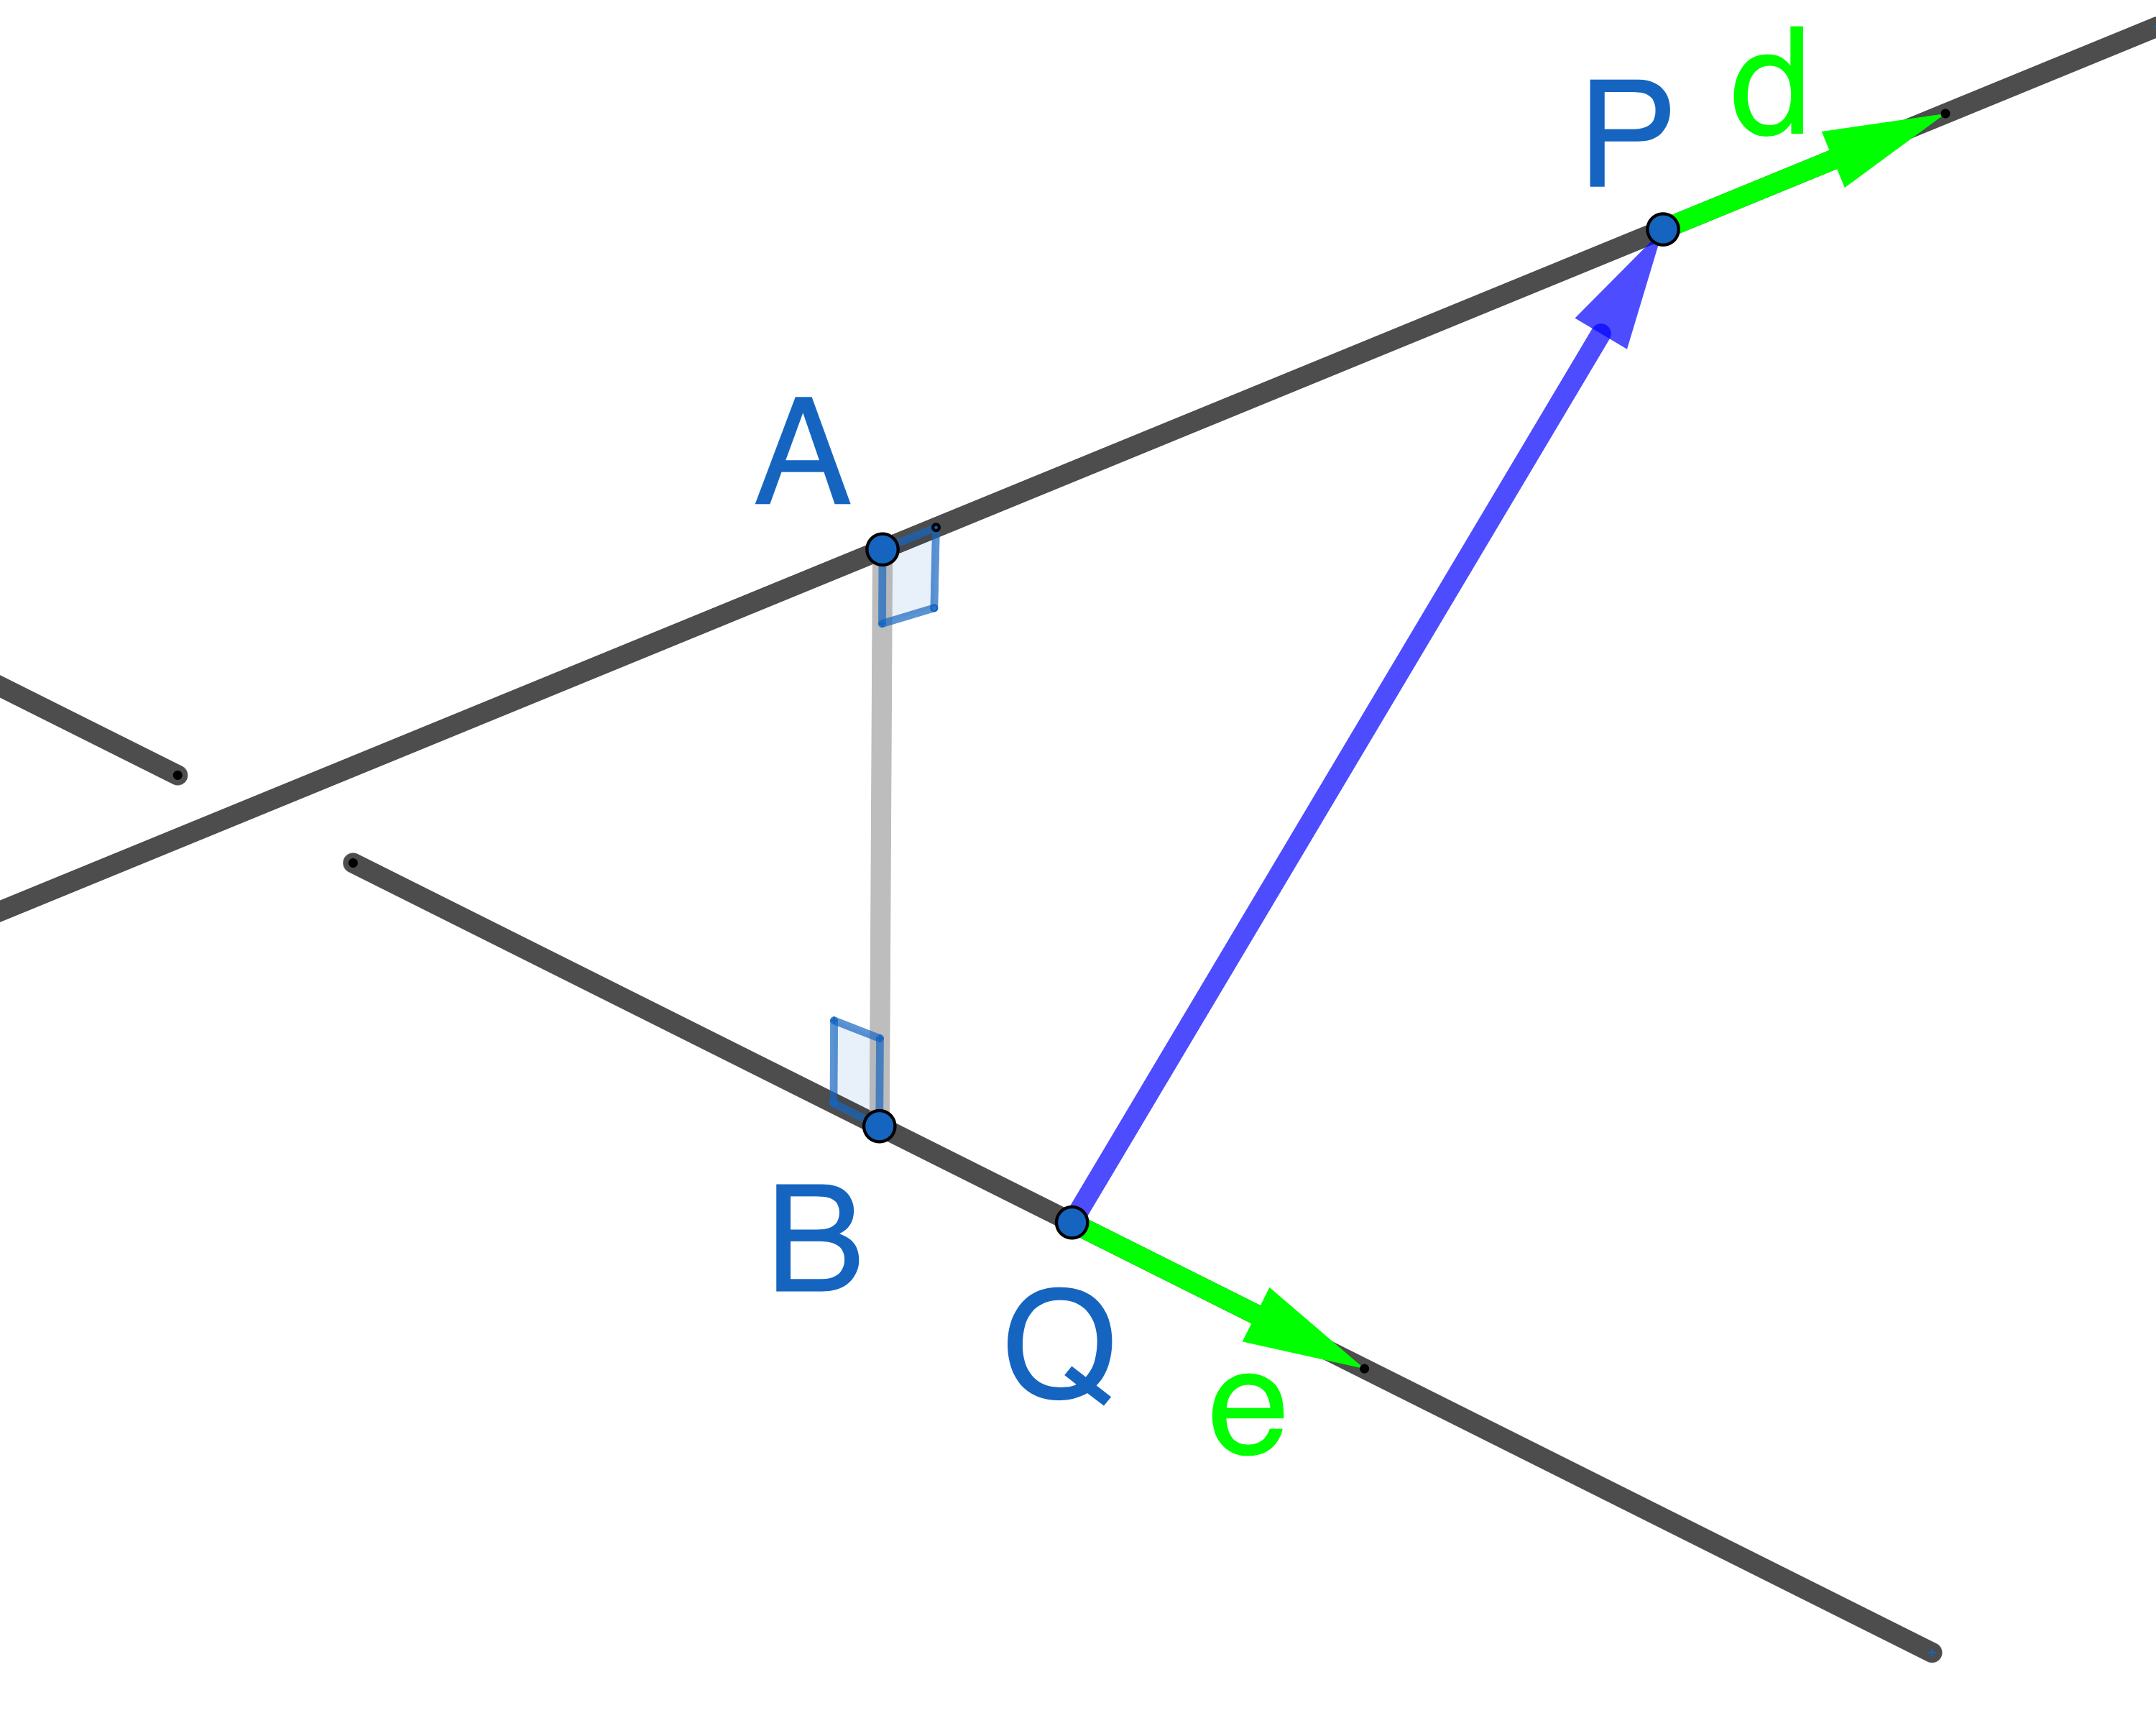
\includegraphics[scale=0.3]{skew-distance1.png}
    \column{0.4\textwidth}
    Suppose we are in $\mathbb{R}^3$.\vfill
    {\bf Key observation:} since
    \begin{equation*}
    \overrightarrow {AB} \perp d\text{ and } \overrightarrow {AB} \perp e
    \end{equation*}
    therefore $d\times e$ is in the same direction as $\overrightarrow{AB}$.
\end{columns}
\end{frame}

\begin{frame}{Closest points on skew lines}
\begin{columns}
    \hspace{-1cm}
    \column{0.5\textwidth}
    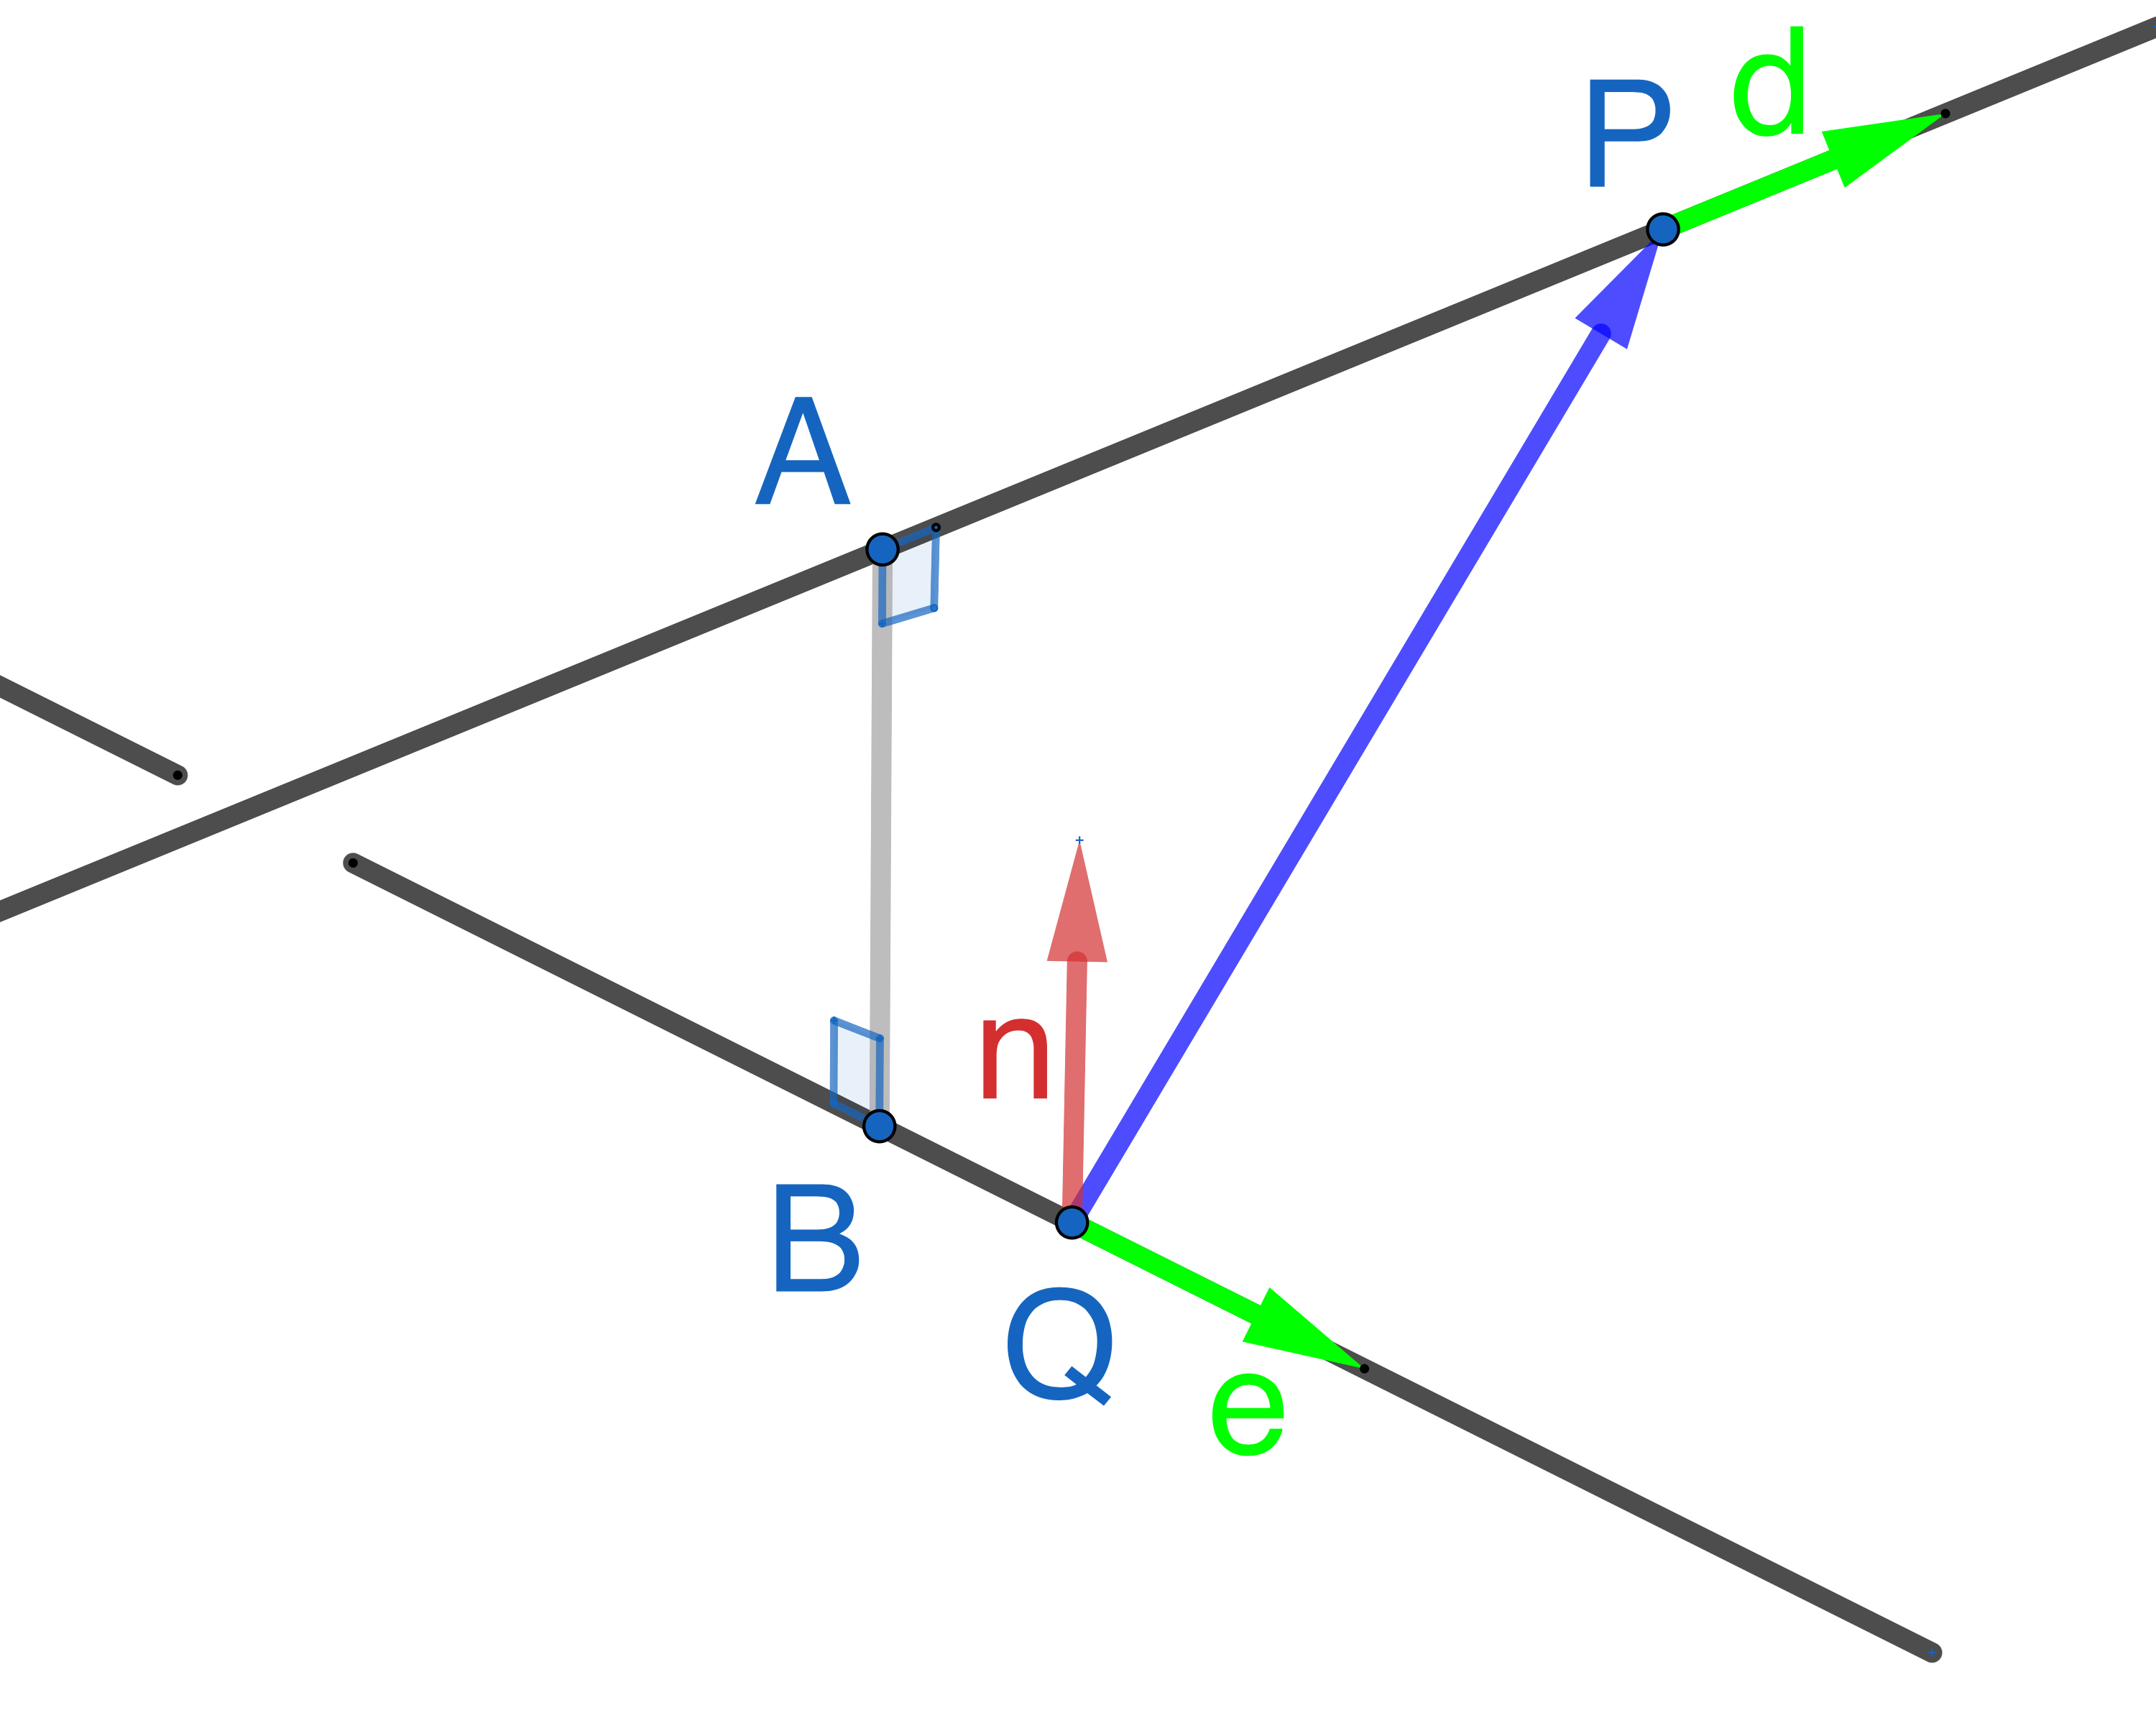
\includegraphics[scale=0.3]{skew-distance2.png}
    \column{0.4\textwidth}
    Let the $n$ be the red vector be the unit vector in direction $\overrightarrow{AB}$ translated to start at $Q$.
    \begin{equation*}
    n =.\frac{d\times e}{\|d\times e\|}
    \end{equation*}
    and so
    \begin{equation*}
    \left\|\overrightarrow{AB}\right\| = n\cdot .\frac{d\times e}{\|d\times e\|}
    \end{equation*}
\end{columns}
\end{frame}

\begin{frame}{Area of a parallelogram}
\begin{columns}
  \column{0.5\textwidth}
  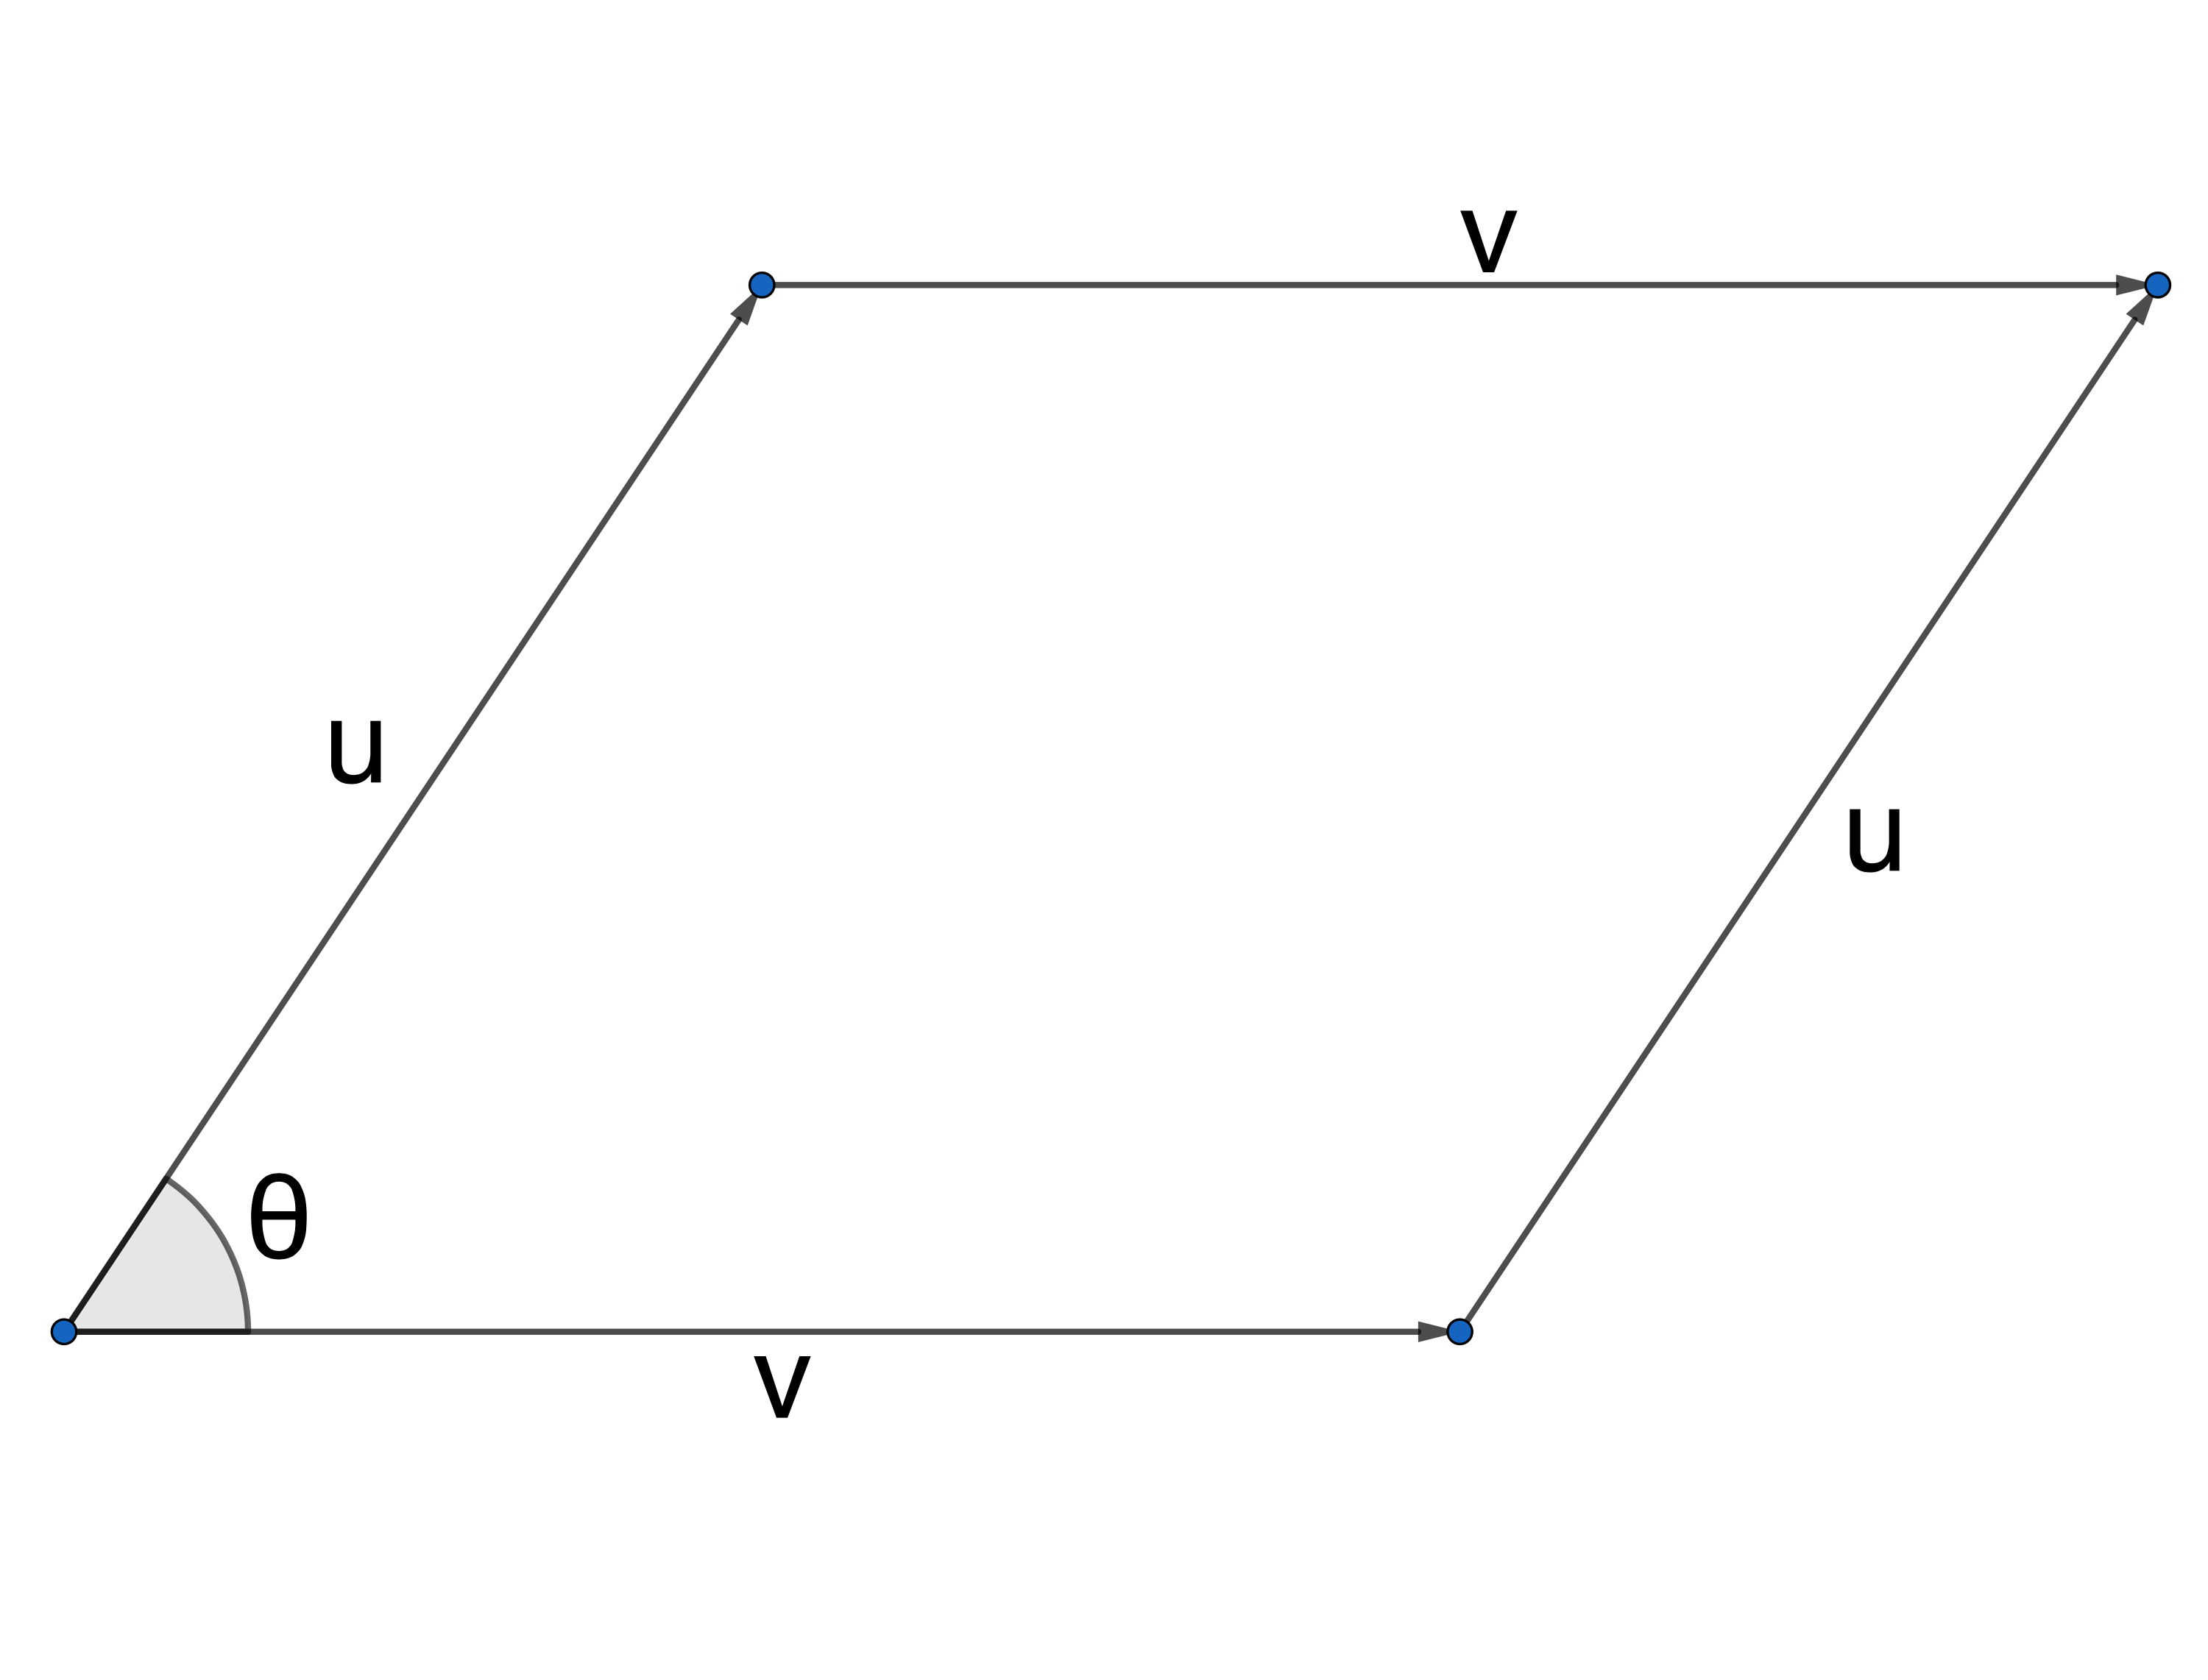
\includegraphics{parallelogram.png}
  \column{0.4\textwidth}
  The area of the parallelogram is:
  \begin{equation*}
  \|u\|\|v\|sin\theta = \|u\times v\|
  \end{equation*}
\end{columns}
\end{frame}

\begin{frame}{Triple scalar (box) product}
\begin{definition}
If $u$, $v$ and $w$ are vectors in $\mathbb{R}^3$ then the \emph{triple scalar product (or box product) of $u$, $v$ and $w$} is
\begin{equation*}
u\cdot (v\times w)
\end{equation*}
\end{definition}
Note that the order of the vectors matters. In fact
\begin{lemma}
\begin{equation*}
u\cdot (v\times w) = \left|
\begin{array}{ccc}
u_1 &v_1 &w_1\\
u_2 &v_2 &w_2\\
u_3&v_3&w_3
\end{array}
\right|
\end{equation*}
which shows that it is the signed volume of the parallelepiped generated by $u$, $v$ and $w$.
\end{lemma}
\end{frame}

\begin{frame}{Examples}
\begin{example}
Find the area of the triangle having vertices
\begin{equation*}
\left[
\begin{array}{c}
3\\
-1\\
2
\end{array}
\right], \left[
\begin{array}{c}
1\\
1\\
0
\end{array}
\right]\text{ and } \left[
\begin{array}{c}
1\\
2\\
-1
\end{array}
\right]
\end{equation*}
\end{example}
\begin{example}
Find the volume of the parallelepiped determined by the vectors
\begin{equation*}
\left[
\begin{array}{c}
2\\
1\\
-1
\end{array}
\right], \left[
\begin{array}{c}
1\\
0\\
2
\end{array}
\right]\text{ and } \left[
\begin{array}{c}
2\\
1\\
1
\end{array}
\right]
\end{equation*}
\end{example}
\end{frame}

\section{Misc}

\begin{frame}
\begin{beamercolorbox}[sep=12pt,center]{part title}
\usebeamerfont{section title}
\insertsection\par
\end{beamercolorbox}
\end{frame}

\begin{frame}{Triangle inequality}
\begin{theorem}
  If $u$ and $v$ are vectors in $\mathbb{R}^n$ then
  \begin{equation*}
    \|u+v\| \leq \|u\|+\|v\|
  \end{equation*}
\end{theorem}\vfill
\begin{theorem}
  If $u$ and $v$ are vectors in $\mathbb{R}^n$ then
  \begin{equation*}
    |\|u\|-\|v\||\leq \|u-v\|
  \end{equation*}
\end{theorem}
\end{frame}

\begin{frame}{The Lagrange identity}
\begin{theorem}
If $u$ and $v$ are in $\mathbb{R}^3$ then
\begin{equation*}
\|u\times v\|^2 = \|u\|^2\|v\|^2-(u\cdot v)^2
\end{equation*}
\end{theorem}
\end{frame}

\begin{frame}{Example}
    \begin{example}
        Find equations for the lines through
        \begin{equation*}
            \left[
            \begin{array}{c}
            1\\
            0\\
            1
            \end{array}
            \right]
        \end{equation*}
        that meet the line
        \begin{equation*}
            \left[
            \begin{array}{c}
            x\\
            y\\
            z
            \end{array}
            \right] = \left[
            \begin{array}{c}
            1\\
            2\\
            0
            \end{array}
            \right]+s \left[
            \begin{array}{c}
            2\\
            -1\\
            2
            \end{array}
            \right]
        \end{equation*}
        at the two points distance three from $(1, 2, 0)$.
    \end{example}
\end{frame}

\begin{frame}{Examples}
    \begin{example}
        The diagonals of a parallelogram bisect each other.
      \end{example}
      \begin{example}
        If $ABCD$ is an arbitrary quadrilateral then the midpoints of the four sides form a parallelogram.
      \end{example}
\end{frame}

\begin{frame}{Examples}
\begin{example}
Find the shortest distance between the following plane and line.
\begin{equation*}
P_1:x-y+2z=2, L_1:\left[
\begin{array}{c}
1\\
1\\
3
\end{array}
\right]+t \left[
\begin{array}{c}
1\\
-1\\
-1
\end{array}
\right]
\end{equation*}
\end{example}
\begin{example}
Find the shortest distance between the following two planes.
\begin{equation*}
P_1:x-y+2z=5, P_2:2x-2y+4z=4
\end{equation*}
\end{example}
\end{frame}

\begin{frame}{Examples}
\begin{example}
Find the distance between the following two lines.
\begin{equation*}
\left[
\begin{array}{c}
x\\
y\\
z
\end{array}
\right] = \left[
\begin{array}{c}
3\\
1\\
-1
\end{array}
\right]+s \left[
\begin{array}{c}
1\\
1\\
-1
\end{array}
\right]\text{ and } \left[
\begin{array}{c}
x\\
y\\
z
\end{array}
\right] = \left[
\begin{array}{c}
1\\
2\\
0
\end{array}
\right] +t \left[
\begin{array}{c}
1\\
0\\
2
\end{array}
\right]
\end{equation*}
\end{example}
\end{frame}

\end{document}